\addtocontents{toc}{\protect}
\section{\texorpdfstring{\MakeUppercase{radiative transfer models and observables of supernovae in active galactic nuclear accretion disks}}{radiative transfer models and observables of supernovae in active galactic nuclear accretion disks}}
\label{sec:sn-rt}

\counterwithin{figure}{section}
\counterwithin{table}{section}


Here we describe the radiative transfer models we apply as post-processing to the three-dimensional hydrodynamic models described in the previous chapter.
The content will be submitted to the \textit{Astrophysical Journal} for publication.
Please cite Cook et al. (2026b) when possible.


\subsection{Methods} \label{sec:methods}

% ======================
% ======================

\subsubsection{Vertical Temperature Profile} \label{subsec:temperature-profile}

The disk models in Ch.~\ref{sec:sn-hydrodynamics} were initialized isothermally by setting the sound speed according to the midplane temperature $\Tmid$ at the SN's radius in a \citet{SirkoGoodman03} disk.
In hydrostatic equilibrium an isothermal disk has a vertical density profile that is Gaussian, which is a good approximation for the temperature in passive disks (those heated by an external source).
Active disks (those internally heated) are much hotter in the midplane and have much more complicated vertical structures, and determining the $T(z)$ dependence is non-trivial.
For this study, we apply a temperature mask over the entire domain for each snapshot of the form
\begin{equation}
\label{eqn:temp-profile}
    T(z) =
    \begin{cases}
	\Tiso & T>\Tmid \\
	\Tmid e^{- \frac{z^2}{2 H_T^2}} & \Tfloor < T < \Tmid \\
	\Tfloor & T<\Tfloor
    \end{cases}
\end{equation}
where $\Tfloor=2000$ K.
We could use simply $\Tiso = \Tmid$, but in practice we find that we need to allow for some flexibility in regions modified by the SN Gaussian in the initial conditions.
As such, we set $\Tiso = (1+\epsilon) \Tmid$, and find empirically that $\epsilon=10^{-2}$ gives acceptable results.
We find the temperature scale height $H_T=1.7\,H$ by root-solving for the profile from the midplane temperature to the effective temperature $\Teff$ using the Eddington approximation
\begin{equation}
	T = \left( \frac{3}{8} \tau + \frac{1}{2} + \frac{1}{4\tau} \right)^{1/4}\ \Teff.
\end{equation}
where we calculate $\tau$ using the Rosseland mean opacity given the vertical disk density profile.
This formulation allows us to bypass regions modified by the SN and only apply the disk profile to zones where the disk is unchanged.


% ======================
% ======================

%
%  Section on Light Curves
%
\subsubsection{Radiative Transfer Post-Processing} \label{subsec:rad-transfer}


We calculate the wavelength-dependent continuum intensity emerging from the hydrodynamic models via post-processing including attenuation from absorption and scattering processes along each column.
The cooling timescale is long compared to the dynamical timescale for our setup, so we can consider the gas to be adiabatic since radiative losses are small.
We solve the following form of the radiative transfer equation,
\begin{equation}\label{eqn:RadTrans}
    \cos\theta \frac{1}{(\kappa_\lambda + \sigma_\lambda)\rho} \frac{dI_\lambda}{dz} = -I_\lambda + S_\lambda,
\end{equation}
where $\theta$ is the direction of propagation, $\kappa_\lambda$ is the opacity due to true absorption, $\sigma_\lambda$ is the scattering opacity, $\rho$ is the volumetric gas density, $I_\lambda$ is the radiation field's intensity, and $S_\lambda$ is the source function.
The presence of scattering calls for an effective source function that depends on the Planck function $B_\lambda$ and the mean intensity $J_\lambda$,
\begin{align}
    S_\lambda &= \frac{\kappa_\lambda B_\lambda + \sigma_\lambda J_\lambda}{\kappa_\lambda + \sigma_\lambda}  \nonumber\\
              &= (1-\omega_\lambda) B_{\lambda} + \omega_\lambda J_\lambda \label{eqn:effective_source}
\end{align}
where $\omega_\lambda = \sigma_\lambda / (\kappa_\lambda + \sigma_\lambda)$ is the single-scattering albedo.
The subscript $\lambda$ indicates quantities with wavelength dependence.
By restricting $\theta$ to be either 0 or $\pi$, we adopt the two-stream approximation which allows the radiation field to travel only upwards ($\Iplus$) or downwards ($\Iminus$), respectively, along the $z$-axis through independent columns of cells located at a given $(x, y)$ position.
First, we tried direct integration like in \citet{Godines+26}, but unlike a protoplanetary disk, an AGN disk is not isothermal and does not allow for this crude integration which lost too much flux in the non-conservative direct integration due to exponentially changing intensities.
Therefore, each column is treated as an isolated stream and is solved using the Feautrier method \citep{Feautrier64,Cannon70}, an implicit method which calculates the mean intensity at each point simultaneously.
%See Appendix \ref{sec:Apdx-Feautrier} for our modification of the method to include scattering and our boundary conditions.
It is appropriate for the general case where extinction occurs via absorption and scattering processes.

This method outlined below forms the core of the \ocotillo code, a multi-wavelength post-processing radiative transfer calculation that we developed for this purpose.

\subsubsubsection{Feautrier method}
\label{sec:Feautrier-method}

To begin, we adopt the two stream Eddington approximation for the radiation field by taking $\theta = 0$ (along z) and $\pi$ (opposite to z) in \eq{eqn:RadTrans}.
This leads to a set of two equations for each stream: $\Iplus_\lambda$ upwards and $\Iminus_\lambda$ downwards, respectively.
With $\alpha_\lambda = \rho(\kappa_\lambda + \sigma_\lambda)$,
\begin{align} 
    \frac{1}{\alpha_\lambda}\frac{d\Iplus_\lambda}{dz} &= -\Iplus_\lambda + S_\lambda \label{eqn:dIpdz}, \\
    -\frac{1}{\alpha_\lambda}\frac{d\Iminus_\lambda}{dz} &= -\Iminus_\lambda + S_\lambda. \label{eqn:dImdz}
\end{align}
The effective source function $S_\lambda$ defined in \eq{eqn:effective_source} is composed of the Planck function
\begin{equation}
    B_{\lambda}(T) = \frac{2hc^2/\lambda^5}{\exp(hc/\lambda k T) - 1},
\end{equation}
and the mean intensity
\begin{equation}
    J_\lambda = \frac{1}{4\pi}\int I_\lambda d\Omega.
\end{equation}
We now drop the subscript $\lambda$ for clarity.
Adding \eq{eqn:dIpdz} to \eq{eqn:dImdz}
\begin{equation}\label{eqn:dIdz}
    \frac{1}{\alpha}\frac{d(\Iplus + \Iminus)}{dz} = - (\Iplus - \Iminus).
\end{equation}
Dividing by two and defining the mean intensity as 
\begin{equation}
    U = \frac{\Iplus + \Iminus}{2}
\end{equation}
and the flux as
\begin{equation}
    V = \frac{\Iplus - \Iminus}{2},
\end{equation}
\eq{eqn:dIdz} simplifies to
\begin{equation}\label{eqn:dUdz=-V}
    \frac{1}{\alpha}\frac{dU}{dz} = -V.
\end{equation}
Subtracting \eq{eqn:dImdz} from \eq{eqn:dIpdz}
\begin{equation}
    \frac{1}{\alpha}\frac{d(\Iplus - \Iminus)}{dz} = - (\Iplus + \Iminus) + 2S.
\end{equation}
Again, dividing by two with the same substitutions and remembering the effective source function \eqp{eqn:effective_source},
\begin{equation}
    \frac{1}{\alpha}\frac{dV}{dz} = -U + (1-\omega) B + \omega J.
\end{equation}
In the two-stream approximation $J=U$ simplifying the previous equation further to
\begin{equation}
    \frac{1}{\alpha}\frac{dV}{dz} = -(1-\omega) U + (1-\omega) B. \\
\end{equation}

Now, we have two equations for the mean intensity $U$ and flux $V$
\begin{align}
    \frac{1}{\alpha}\frac{dU}{dz} =& -V; \label{eqn:dUdz} \\
    \frac{1}{\alpha}\frac{dV}{dz} =& (1-\omega)(B-U). \label{eqn:dVdz}
\end{align}
Substituting $V$ into the second leaves one equation in $U$,
\begin{equation}\label{eqn:ddU/ddz}
    \frac{d}{dz} \left( \frac{1}{\alpha} \frac{dU}{dz} \right) = -\alpha(1-\omega)(B-U).
\end{equation}

Next, we discretize $U$ onto a uniform grid (i.e., $\Delta z =$ const).
To evaluate the point $i$ using centered derivatives, we define the fluxes $\phi$ at the half-grid points
\begin{equation}\label{eqn:U_i-discrete}
    \frac{\Delta}{\Delta z} \left( \frac{1}{\alpha_i}\frac{\Delta U_i}{\Delta z} \right) = \frac{\phi_{i+\sfrac{1}{2}} - \phi_{i-\sfrac{1}{2}}}{\Delta z}
\end{equation}
where the fluxes at the cell interfaces $i\pm\sfrac{1}{2}$ are calculated using the forward and backward points
\begin{eqnarray}
    \phi_{i+\sfrac{1}{2}} = \frac{1}{\alpha_{i+\sfrac{1}{2}}} \frac{(\Uipone - \Ui)}{\Delta z}, \\
    \phi_{i-\sfrac{1}{2}} = \frac{1}{\alpha_{i-\sfrac{1}{2}}} \frac{(\Ui - \Uimone)}{\Delta z}.
\end{eqnarray}

Using \eq{eqn:U_i-discrete} to replace the left-hand side of \eq{eqn:ddU/ddz}
\begin{equation}
      \frac{1}{\alpha_{i+\sfrac{1}{2}}} \frac{(\Uipone - \Ui)}{\Delta z} 
    - \frac{1}{\alpha_{i-\sfrac{1}{2}}} \frac{(\Ui - \Uimone)}{\Delta z}  
    = - \alpha_i (1 - \omega_i)(B_i - \Ui) \Delta z
\end{equation}
and collecting terms in $U$
\begin{equation}
    \frac{1}{\alpha_{i+\sfrac{1}{2}}} \Uipone - \left[ \frac{1}{\alpha_{i+\sfrac{1}{2}}}+ \frac{1}{\alpha_{i-\sfrac{1}{2}}} + \xi_i  \right] \Ui + \frac{1}{\alpha_{i-\sfrac{1}{2}}} \Uimone  = - \xi_i B_i,
\end{equation}
where $\xi_i = \alpha_i (1 - \omega_i) \Delta z^2$, we arrive at a form that can be constructed as a system of equations for each $i$ in matrix form with $\Ui$ along the diagonal and the $\Uimone$ and $\Uipone$ terms falling along the left and right off-diagonals, respectively, 
\begin{equation}
    a_i \Uipone + b_i \Ui + c_i \Uimone = d_i, \label{eqn:system-in-U_i}
\end{equation}
where
\begin{eqnarray}
    a_i &=& 1/\alpha_{i+\sfrac{1}{2}} \\
    c_i &=& 1/\alpha_{i-\sfrac{1}{2}} \\
    b_i &=& -a_i - c_i - \xi_i \\
    d_i &=& - \xi_i B_i
\end{eqnarray}
This tridiagonal matrix can be solved using standard methods for the mean intensity at each point.
Then, using \eq{eqn:dUdz=-V} we can solve for the flux $V$ and upwards $\Iplus$ and downwards $\Iminus$ intensities using the definitions for $U = \Iplus + \Iminus$ and $V = \Iplus - \Iminus$.

The quantities at the domain boundaries represent the observable radiation field.
The flux defined in the two-stream approximation is converted into the flux density by $F_\lambda = 2 \pi V_\lambda$.

\subsubsection{Boundary Conditions}
We set the radiation field at the vertical boundaries to be outflow only.
Considering $U = (\Iplus + \Iminus) / 2$ and $V = (\Iplus + \Iminus) / 2$, outflow boundaries imply the lower boundary at $z=-L/2$ has an upward intensity $\Iplus=0$, such that $U(z=0) = \Iminus/2$ and $V(z=0)=-\Iminus/2$, and thus $U=-V$.

In order to match the second order in $\Delta z$ we expand $U$ close to the boundary in a Taylor series
\begin{equation}
    U_{\sfrac{1}{2}} = U_0 + \frac{\Delta \tau}{2} \left. \frac{dU}{d\tau} \right|_0 + \frac{\Delta \tau^2}{8} \left. \frac{d^2U}{d\tau^2}\right|_0
\end{equation}
Substituting $U_{\sfrac{1}{2}} = (U_0 + U_1)/2$,
\begin{equation}
    \frac{U_1 + U_2}{2} = U_0 + \frac{\Delta \tau}{2} \left. \frac{dU}{d\tau} \right|_0 + \frac{\Delta \tau^2}{8} \left. \frac{d^2U}{d\tau^2}\right|_0.
\end{equation}
Using \eq{eqn:dUdz} -- \eq{eqn:ddU/ddz}, we have the first and second derivatives of $U$ in $\tau$.
Evaluating these at $z=0$
\begin{align}
    \left. \frac{dU}{d\tau} \right|_0 &= U_0 \text{  (since}\ U_0=-V_0 \text{ for } \Iplus=0), \\
    \left. \frac{d^2U}{d\tau^2}\right|_0 &= (1-\omega_0)(U_0-B_0),
\end{align}
and the expression for $U_{\sfrac{1}{2}}$ becomes
\begin{equation}
    \frac{U_0 + U_1}{2} = U_0 + \frac{\Delta \tau}{2} U_0 + \frac{\Delta \tau^2}{8} (1-\omega_0)(U_0-B_0).
\end{equation}
Collecting terms in $U_i$
\begin{equation}
    U_0 \left[ -1-\Delta \tau - \frac{\Delta \tau^2}{4}(1-\omega_0) \right] + U_1 = - \frac{\Delta \tau^2}{4}(1-\omega_0)B_0.
\end{equation}
Reintroducing $\Delta \tau =\alpha \Delta z$,
\begin{equation}
    U_0 \left[ -1-\alpha_0\Delta z - \frac{\alpha_0^2\Delta z^2}{4}(1-\omega_0) \right] + U_1 = - \frac{\alpha_0^2\Delta z^2}{4}(1-\omega_0)B_0.
\end{equation}
Dividing by $\alpha_0$, the coefficients as defined in \eq{eqn:system-in-U_i} have the quantities
\begin{eqnarray}
    a_0 &=& 0, \\
    b_0 &=& -1\left[ \frac{1}{\alpha_0} + \Delta z + \frac{\alpha_0 \Delta z^2}{4}(1-\omega_0) \right], \\
    c_0 &=& 1/\alpha_{0}, \\
    d_0 &=& - \frac{\alpha_0 \Delta z^2}{4}(1-\omega_0) B_0.
\end{eqnarray}
At the upper boundary $z=L/2$, the downward intensity $\Iminus=0$ leading to $U_N=V_N$.
The same exercise as above results in the coefficients
\begin{eqnarray}
    a_N &=& 1/\alpha_N, \\
    b_N &=& -1\left[ \frac{1}{\alpha_N} + \Delta z + \frac{\alpha_N \Delta z^2}{4}(1-\omega_N) \right], \\
    c_N &=& 0, \\
    d_N &=& - \frac{\alpha_N \Delta z^2}{4}(1-\omega_N) B_N.
\end{eqnarray}
We call attention here to an important subtlety, that the Taylor expansion near the boundary gives the coefficients the same order in $\alpha$ and $\Delta z$ as those for the rest of the domain.

\subsubsection{Opacities}
Given the density and temperature of a zone, we solve for the populations of neutral hydrogen H, ionized hydrogen $\Hplus$, the negative hydrogen ion $\Hminus$, and free electrons.
The neutral and negative ion species absorb radiation when an electron is stripped away through the bound-free (bf) ionization process, $\kappa(\text{H}_\text{bf})$ and $\kappa({\Hminus_\text{bf}})$ respectively, and the positive and negative hydrogen ions absorb photons via free-free (ff), or Bremsstrahlung, interactions with free electrons, noted as $\kappa (\text{H}_\text{ff})$ and $\kappa (\Hminus_\text{ff})$.
%We calculate the combined continuous absorption from these processes, following \citet{Gray76,Gray21}, as
%\begin{align}
%       \kappa_\lambda =& \biggl\{ \bigl[ \kappa(\text{H}_\text{bf}) + \kappa(\text{H}_\text{ff}) + \kappa(\text{H}^-_\text{bf}) \bigr] (1 - 10^{-\chi \theta}) \nonumber \\
%		    &+ \kappa(\text{H}^-_\text{ff}) \biggr\} \frac{1}{1 + \Phi_\text{H}(T) / P_\text{e}}  + \kappa(\text{e}^-).
%\end{align}
%The factor $1-10^{-\chi\theta}$ accounts for the stimulated emission of H and $\Hminus$ with $\theta = 5040 / T\ \text{eV}^{-1}$ and $\chi(\lambda) = 1.2398 \times 10^4 / \lambda\ \text{eV}$ when $T$ is in Kelvin and $\lambda$ is in \r{a}ngstr\"om.
%The ionization state $\Phi_\text{H}(T)$ is given by the Saha equation, and $P_\text{e}$ is the partial pressure due to free electrons.
%Though scattering processes in general can be wavelength-dependent, the scattering coefficient for free electrons $\sigma$ is wavelength-\emph{independent}, but it is proportional to the ratio between the number densities of ionized hydrogen $n_\text{HII}$ to total hydrogen $n_\text{H}$, $\sigma = 0.6648 \times 10^{-24} \,n_\text{HII} / n_\text{H}$.
%This model ignores line opacities and only treats the continuum emission.
%See Appendix \ref{sec:Apdx-Opacities} for full descriptions of the absorption and scattering coefficients.

We calculate the continuous opacity with contributions from bound-free and free-free interactions with neutral hydrogen $\kappa({\rm H})$ and the negative hydrogen ion $\kappa({\rm H^-})$ and electron scattering $\kappa({\rm e})$ following \citet{Gray21}.
This model currently ignores line opacities and only treats the continuum emission.
We adopt their convention for representing the thermal gas energy $\theta = 5040/T\ {\rm eV}^{-1}$ where $T$ is the gas temperature.
The neutral bound-free absorption is 
\begin{equation}\label{eqn:kappaHIbf}
    \kappa({\rm H_{bf}}) = \sigma_0 \lambda^3  \left[ \sum_{n=1}^{m-1} \frac{g_{\rm bf}}{n^3}10^{-\theta \chi_n} + \frac{\rm log_{10}(e)}{2\theta I} \left(10^{-\chi_m \theta} - 10^{-I\theta} \right) \right]
\end{equation}
where $\sigma_0 = 1.0449 \times 10^{-26}$ when $\lambda$ has units \AA, $\chi_{n} = I(1-1/n^2)$ eV is the excitation potential for a bound electron in level $n$, $I=13.598$ eV is the energy required to ionize an electron from the hydrogen atom in the ground state.
The Uns\"old approximation is used for calculating contributions from levels $m=[6, \infty)$ represented by the second term in the square brackets.

The bound-free Gaunt factor $g_{\rm bf}$ is given by
\begin{equation}\label{eqn:gauntHIbf}
    g_{\rm bf} = 1 - \frac{0.3456}{(\lambda R)^{1/3}} \left( \frac{\lambda R}{n^2} - \frac{1}{2} \right)
\end{equation}
with $\lambda$ in \AA and the Rydberg constant for hydrogen $R = 1.09678 \times 10^{-3} / \lambda \ {\text{\AA}^{-1}}$ such that the product $\lambda R$ is dimensionless. Neutral hydrogen free-free absorption is
\begin{equation}\label{eqn:kappaHIff}
    \kappa({\rm H_{ff}}) = \sigma_0 \lambda^3 g_{\rm ff} \frac{\rm log_{10}(e)}{2\theta I} 10^{-I\theta}
\end{equation}
with $\lambda$ in units of \AA and where $\alpha_0$ is as above in Eqn. \ref{eqn:kappaHIbf}. The free-free Gaunt factor $g_{\rm ff}$ for hydrogen is
\begin{equation}
    g_{\rm ff} = 1 + \frac{0.3456}{(\lambda R)^{1/3}} \left( \frac{\rm log_{10}(e)}{\theta \chi_{\lambda}} + \frac{1}{2} \right)
\end{equation}
where $\chi_{\lambda} = 1.2398 \times 10^4 / \lambda$ eV, with $\lambda$ in units of \AA, is the photon energy.

Negative hydrogen ions contribute substantially to the opacity in the solar photosphere.
The photospheric temperature of the \citet{SirkoGoodman03} disk at 1000 $\Rs$ roughly matches this temperature for a disk around an SMBH with $\Mbh=10^8\,\Msun$.
We incorporate both the bound-free and free-free components to reproduce the proper disk opacities.
According to measurements by \citet{Wishart79}, the cross section to the bound-free component between 2250 \AA and 15\,000 \AA in units of $10^{-17}$ cm$^2$ per H$^-$ ion is
\begin{equation}
    \sigma_{\rm bf}(\rm H^-) = \sigma_0 + \sigma_1 \lambda + \sigma_2 \lambda^2 + \sigma_3 \lambda^3 + \sigma_4 \lambda^4 + \sigma_5 \lambda^5 + \sigma_6 \lambda^6.
\end{equation}

The stimulated emission is included and the constants have the values
\begin{align}
    \alpha_0 &= +0.1199654, \\
    \alpha_1 &= -1.18267 \times 10^{-6}, \\
    \alpha_2 &= +2.64243 \times 10^{-7}, \\
    \alpha_3 &= -4.40524 \times 10^{-11}, \\
    \alpha_4 &= +3.23992 \times 10^{-15}, \\
    \alpha_5 &= -1.39568 \times 10^{-19}, \\
    \alpha_6 &= +2.78701 \times 10^{-24}
\end{align}
when $\lambda$ is in \AA.
Then, the bound-free opacity for the negative hydrogen ion is
\begin{equation}
    \kappa({\rm H^-_{bf}}) = 4.158 \times 10^{-10} \, \sigma({\rm H^-_{bf}}) \, P_{\rm e} \, \theta^{5/2} \, 10^{I\, \theta} \\
\end{equation}
where $P_{\rm e}$ is the partial electron pressure and with $I = 0.754$ eV.
The numerical factor includes a conversion to units of cm$^{-2}$ per neutral hydrogen atom.

Absorption due to the H$^{-}$ free-free process was measured by \citet{BellBerrington87} between 2600 and 113,900 \AA{} in the range $\theta = 0.5 - 2.0$ ($T = 10\,000 - 2500 K)$ and takes the form
\begin{equation}
    \kappa({\rm H_{ff}^-}) = 10^{-26} \, P_{\rm e} \, 10^{f_0 + f_1 \, \log_{10} \theta + f_2 \, \log_{10}^2 \theta}
\end{equation}
in units of cm$^2$ per neutral hydrogen atom, which includes the stimulated emission factor. The $f_i$ components of the polynomial expression are
\begin{align}
    f_0 &= -2.2763 - 1.6850 \, \log_{10} \lambda + 0.76661 \, \log_{10}^2 \lambda - 0.0533464 \, \log_{10}^3 \lambda \\
    f_1 &= +15.2827 - 9.2846 \, \log_{10} \lambda + 1.99381 \, \log_{10}^2 \lambda - 0.142631 \, \log_{10}^3 \lambda \\
    f_2 &= -197.789 + 190.266 \, \log_{10} \lambda - 67.9775 \, \log_{10}^2 \lambda + 10.6913 \, \log_{10}^3 \lambda - 0.625151 \, \log_{10}^4 \lambda
\end{align}
when $\lambda$ is in \AA. The disk midplane and supernova are both fully ionized, and in this state electron scattering dominates.

The scattering cross-section in units of cm$^{2}$ per hydrogen atom is 
\begin{equation}
\kappa(\text{e}^-) = 0.6648 \times 10^{-24} \frac{n_{\rm e}}{n_{\rm H}}  \\
\end{equation}
where $n_{\rm e}$ and $n_{\rm H}$ are the number densities of electrons and hydrogen atoms, respectively.

Some of the expressions stated above were normalized per neutral hydrogen atom. We convert them into units of per hydrogen atom using Saha's equation to account for the ionization state. Thus, the total absorption coefficient we use in our radiative transfer calculation is 
\begin{equation}
	\label{eqn:total-kappa}
	\kappa_{\lambda} = \biggl\{ \Bigl[ \kappa({\rm H_{bf}}) + \kappa({\rm H_{ff}}) + \kappa({\rm H^-_{bf}}) \Bigr] (1-10^{\chi_\lambda \theta}) + \kappa({\rm H_{ff}^-}) \biggr\} \times \frac{1}{1-n_{\rm HII}/n_{\rm HI}} + \kappa({\rm e^-})
\end{equation}
where $\chi_\lambda = 1.2398 \times 10^4/\lambda\text{eV}$ when $\lambda$ is in \AA.

\begin{figure}
    \centering
    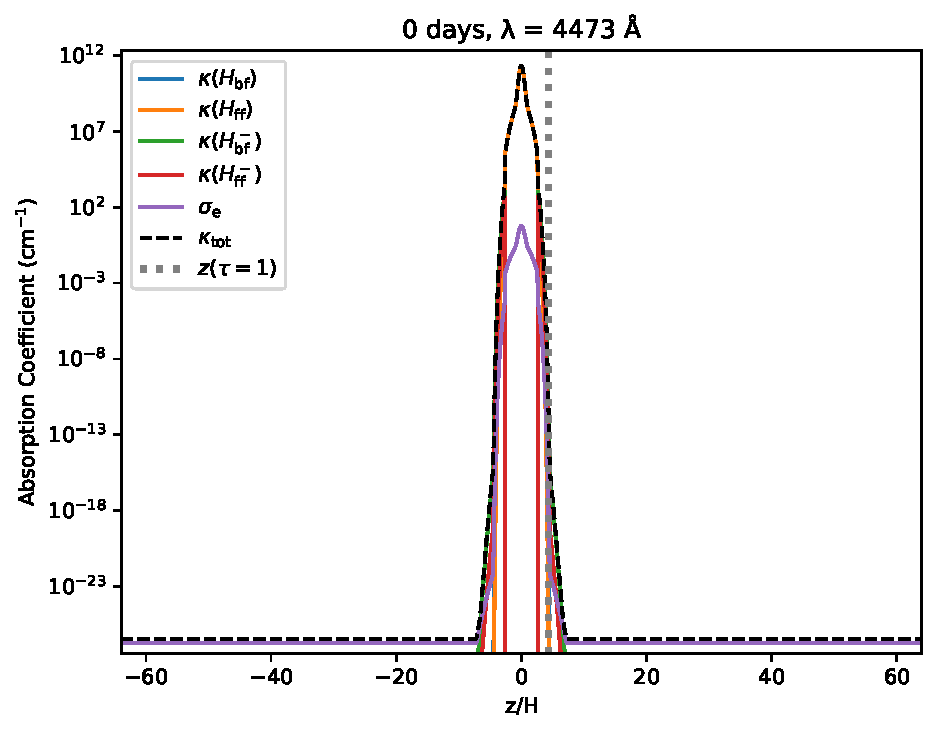
\includegraphics[width=1.0\textwidth]{ch_snrt_figs/opacity_480x480_w4473_0000.pdf}
	\caption[Vertical opacity profiles for initial conditions]{Opacity profiles from model \code{r1e3-z0h} showing contributions from each component in \eq{eqn:total-kappa} for the column passing through the center of the SN for the initial conditions.}
\label{fig:opacity-profile0}
\end{figure}

\begin{figure}
    \centering
    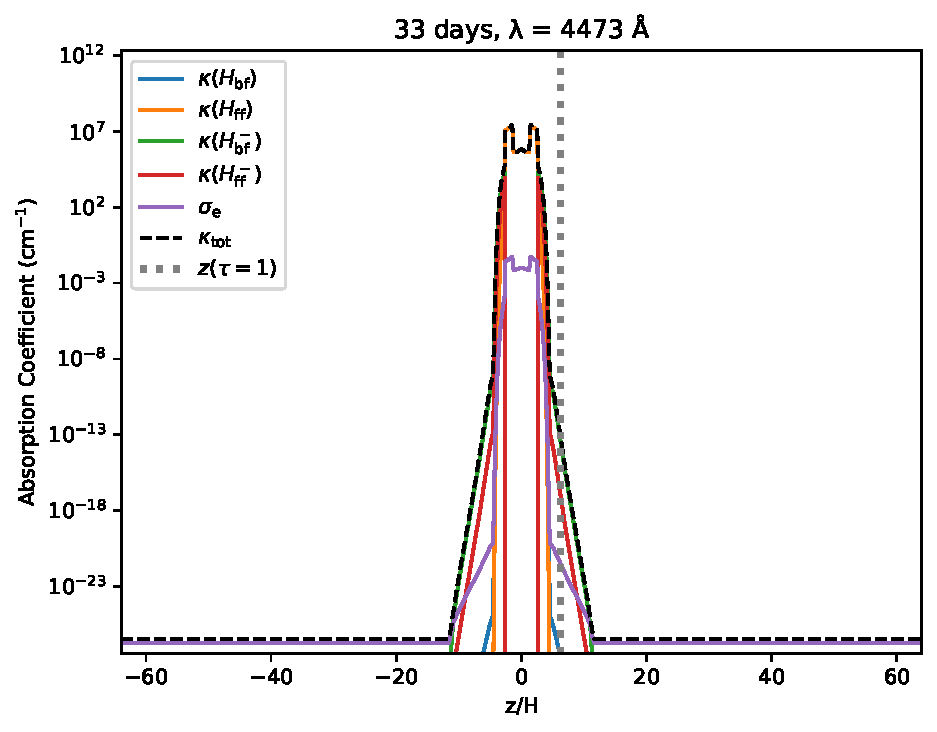
\includegraphics[width=1.0\textwidth]{ch_snrt_figs/opacity_480x480_w4473_0013.pdf}
	\caption[Vertical opacity profiles at shock breakout]{Vertical opacity profiles at shock breakout.}
	\label{fig:opacity-profile13}
\end{figure}

\begin{figure}
    \centering
    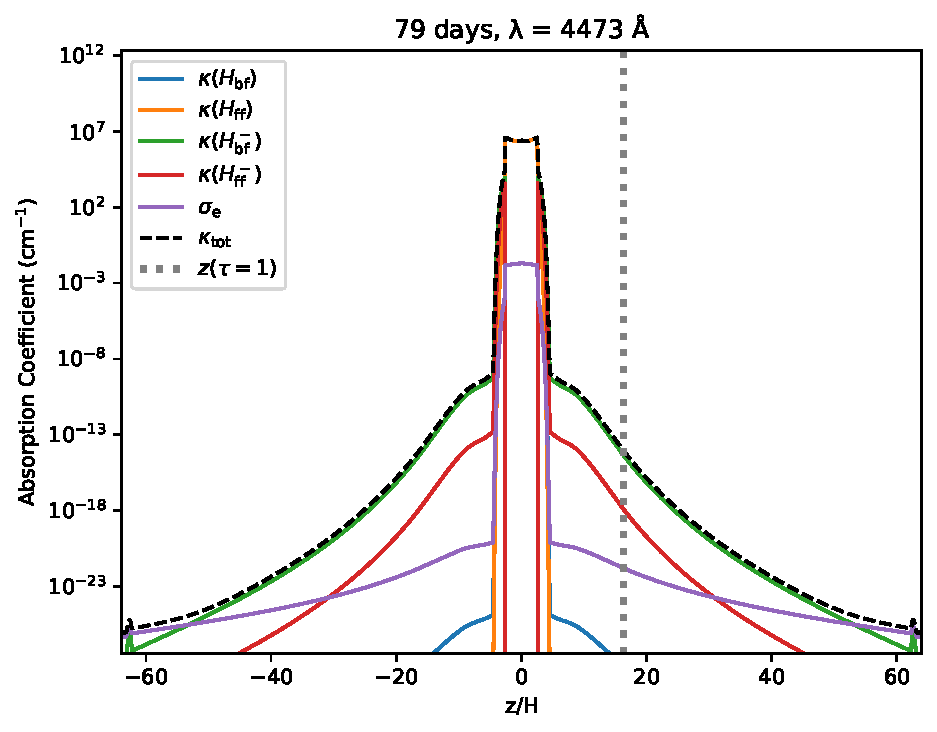
\includegraphics[width=1.0\textwidth]{ch_snrt_figs/opacity_480x480_w4473_0031.pdf}
	\caption[Vertical opacity profiles in final snapshot]{Vertical opacity profiles in the snapshot before the shock leaves the domain.}
	\label{fig:opacity-profile31}
\end{figure}

When the ionization fraction becomes large (i.e., $1 - n_\text{HII}/n_\text{HI}>10^{-2}$), we switch to using the following expression for the free-free absorption component as a function of frequency $\nu$
\begin{equation}
	\kappa_{\nu}(\text{H}_\text{ff}) \rho = \frac{4e^6}{3\, h\, c\, \me^2} \left( \frac{2\pi \me}{3kT} \right)^{1/2} \ \gff\, \nElec\, \nI\, Z^2\, \nu^{-3}\,\left[ 1 - \exp \left(-\frac{h\nu}{kT}\right) \right],
\end{equation}
where
\begin{equation}
    \gff \approx \rm{ln} \bigg( \exp \bigg\{ 5.960 - \frac{\sqrt{3}}{\pi} \ ln \bigg[ \frac{\nu}{10^9\ \rm{Hz}} \bigg( \frac{T}{10^4\ \rm{K}} \bigg)^{-3/2} \bigg] \bigg\} + e \bigg)
\end{equation}
is the Gaunt quantum mechanical correction factor, and the final term $e$ is Napier's constant.
Since this expression is for absorption with units cm$^{-1}$, we take it out of \eq{eqn:total-kappa} and add it directly to our calculation of $\alpha_\lambda$. 

\Fig{fig:opacity-profile0}, \Fig{fig:opacity-profile13}, and \Fig{fig:opacity-profile31} show the opacity profiles for our fiducial model at $R=10^3\,\Rs$ and $z=0H$ for each term in \eq{eqn:total-kappa} for the central wavelength in our range $\lambda=4473\,\text{\AA}$ at the initial conditions, shock breakout, and the snapshot before the shock leaves the $z$ boundary.
The vertical dotted line shows the photosphere ($\tau=1$) when observed from the positive $z$-direction.
At $t=0$ days, the disk midplane is dominated by $\kappa(\text{H}_\text{bf})$ and $\sigma_\text{e}$, but the disk photosphere at $z=5H$ is dominated by free-free absorption from $\kappa(\text{H}_\text{ff})$ and $\kappa(\text{H}_\text{ff}^-)$.
At $t=31$ days when the SN shock passes $z=5H$ and the light curve in \Fig{fig:all_lcs} rises, $\kappa(\text{H}_\text{bf})$ becomes the dominant opacity source.
At $t=76$ days, when the shock reaches the domain boundary, the opacity at the photosphere is still dominated by $\kappa(\Hminus_\text{bf})$ followed by $\kappa(\text{H}_\text{ff})$, which contributes a relatively small amount.

In \Fig{fig:UVIpIm-0}, \Fig{fig:UVIpIm-13}, and \Fig{fig:UVIpIm-31} we show the vertical profiles for the core values calculated with the Feautrier method in the \ocotillo code -- the mean intensity $U$, flux $V$, upward intensity $\Iplus$, and downward intensity $\Iminus$ -- for the same times and wavelength as in \Fig{fig:opacity-profile0}, \Fig{fig:opacity-profile13}, and \Fig{fig:opacity-profile31}, respectively, along the central column that passes through the SN.
The strong bump in the middle of the initial conditions for $U$, $\Iplus$, and $\Iminus$ is generated by the SN perturbation, and the small bump at the base is caused by the accretion disk.
The curve for $V$ represents the flux of energy being passed to the cells on either side of a given point, meaning an observer sees the value at the boundaries.
The center is bright due to the SN, but the flux drops quickly as the disk absorbs the radiation.
Moving further outwards, the radiation is emitted again at the disk edge and streams freely towards the boundaries.
When the shock breaks out at $t=33$ days, $V$ increases until it reaches its maximum when the shock is near the $z$-boundary at $t=79$ days.

\begin{figure}
	\centering
	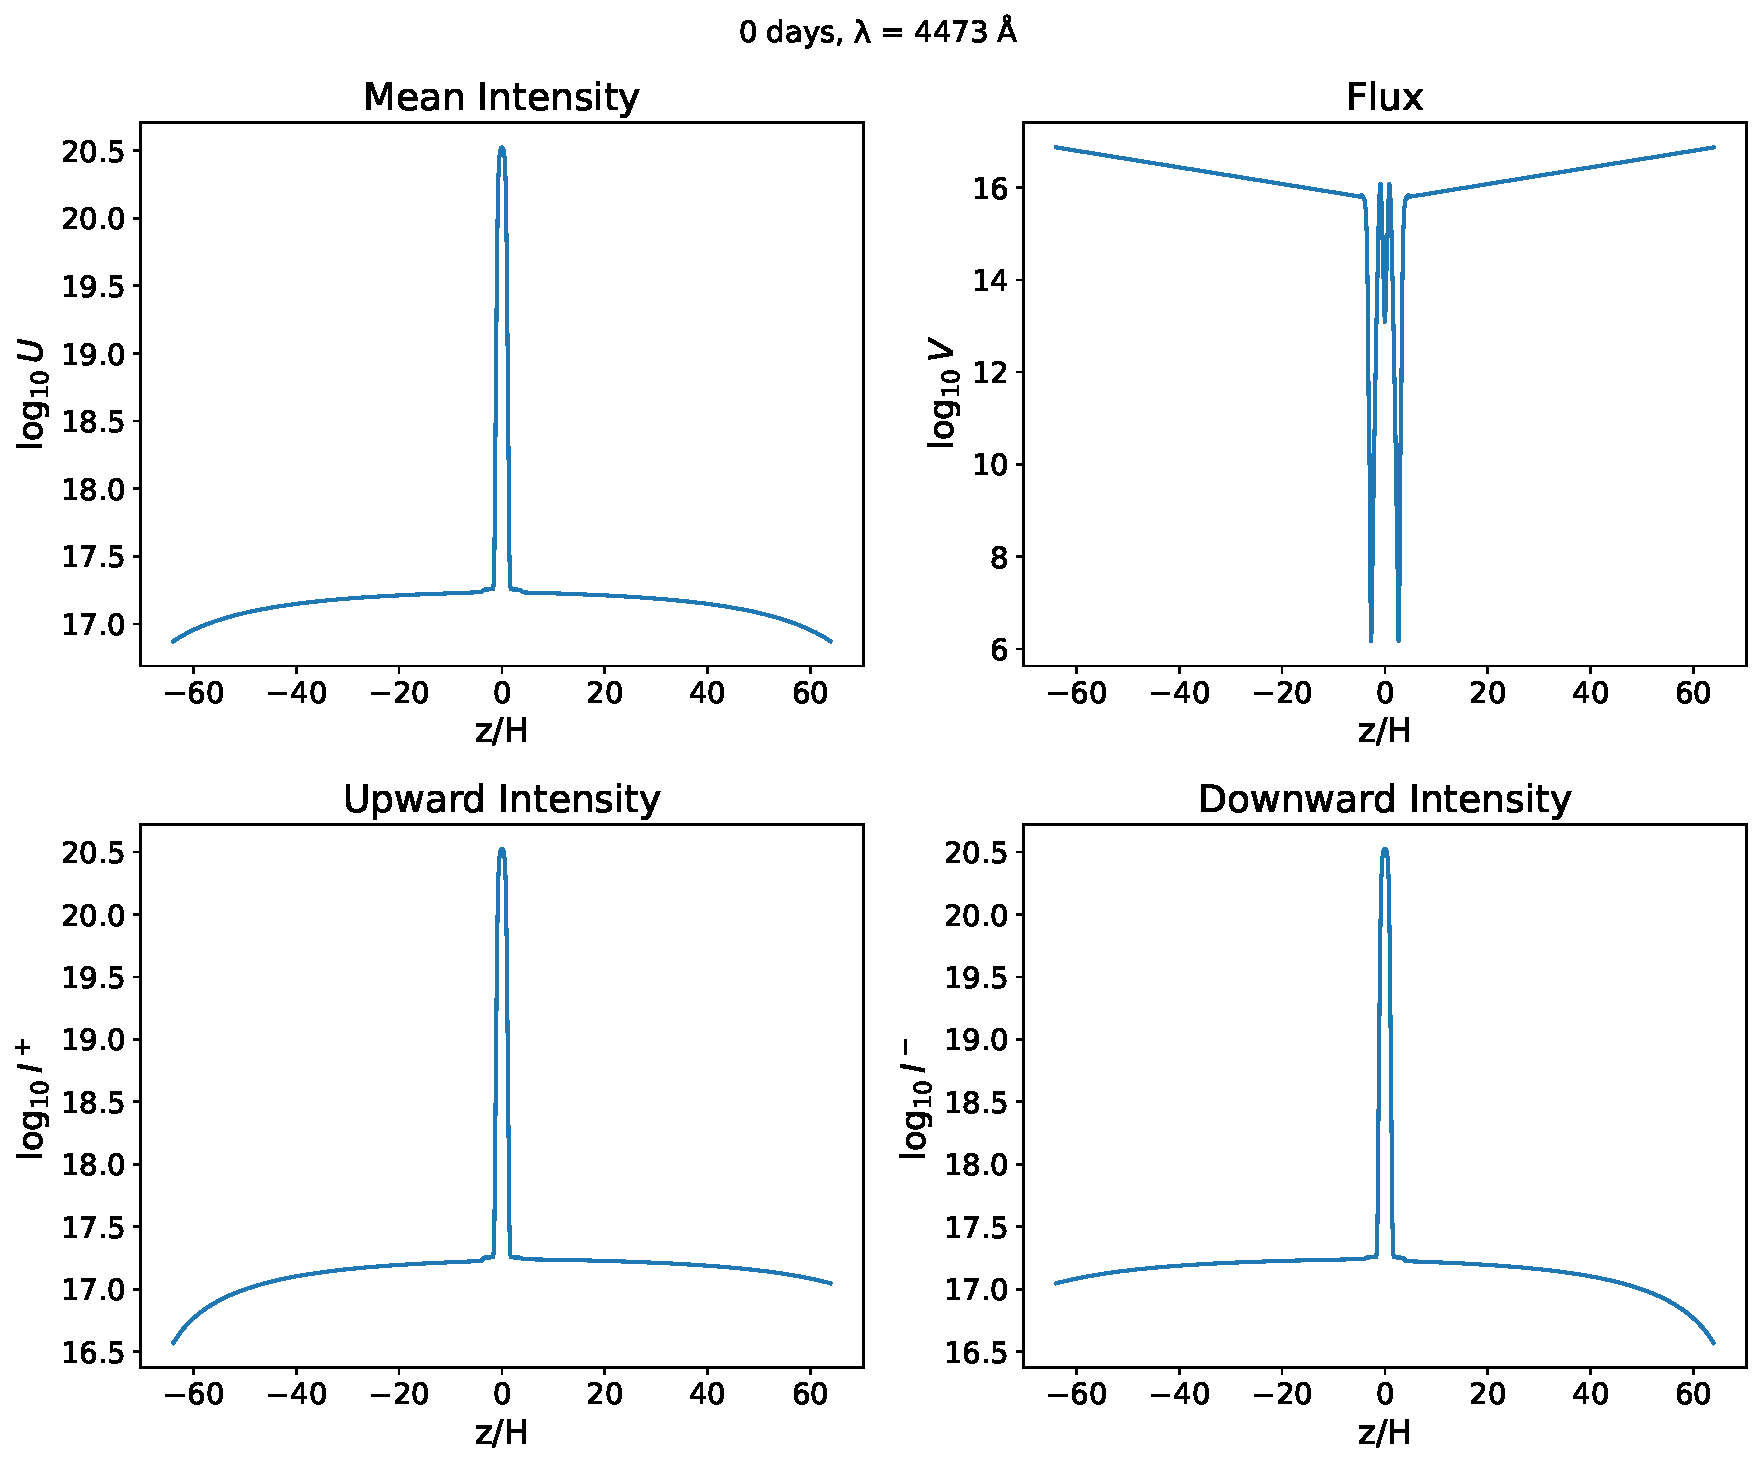
\includegraphics[width=1\textwidth]{ch_snrt_figs/intensity_480x480_w4473_0000.pdf}
	\caption[Feautrier Solutions from \ocotillo for the fiducial model \texttt{r1e3\_z0h} at 0 days]{Feautrier solutions. Mean intensity (upper left), flux (upper right), and upward intensity (lower left), and downward intensity (lower right)when applied to our density and temperature initial conditions for the central wavelength in our array $\lambda=4473\,\text{\AA}$.}
	\label{fig:UVIpIm-0}
\end{figure}

\begin{figure}
	\centering
	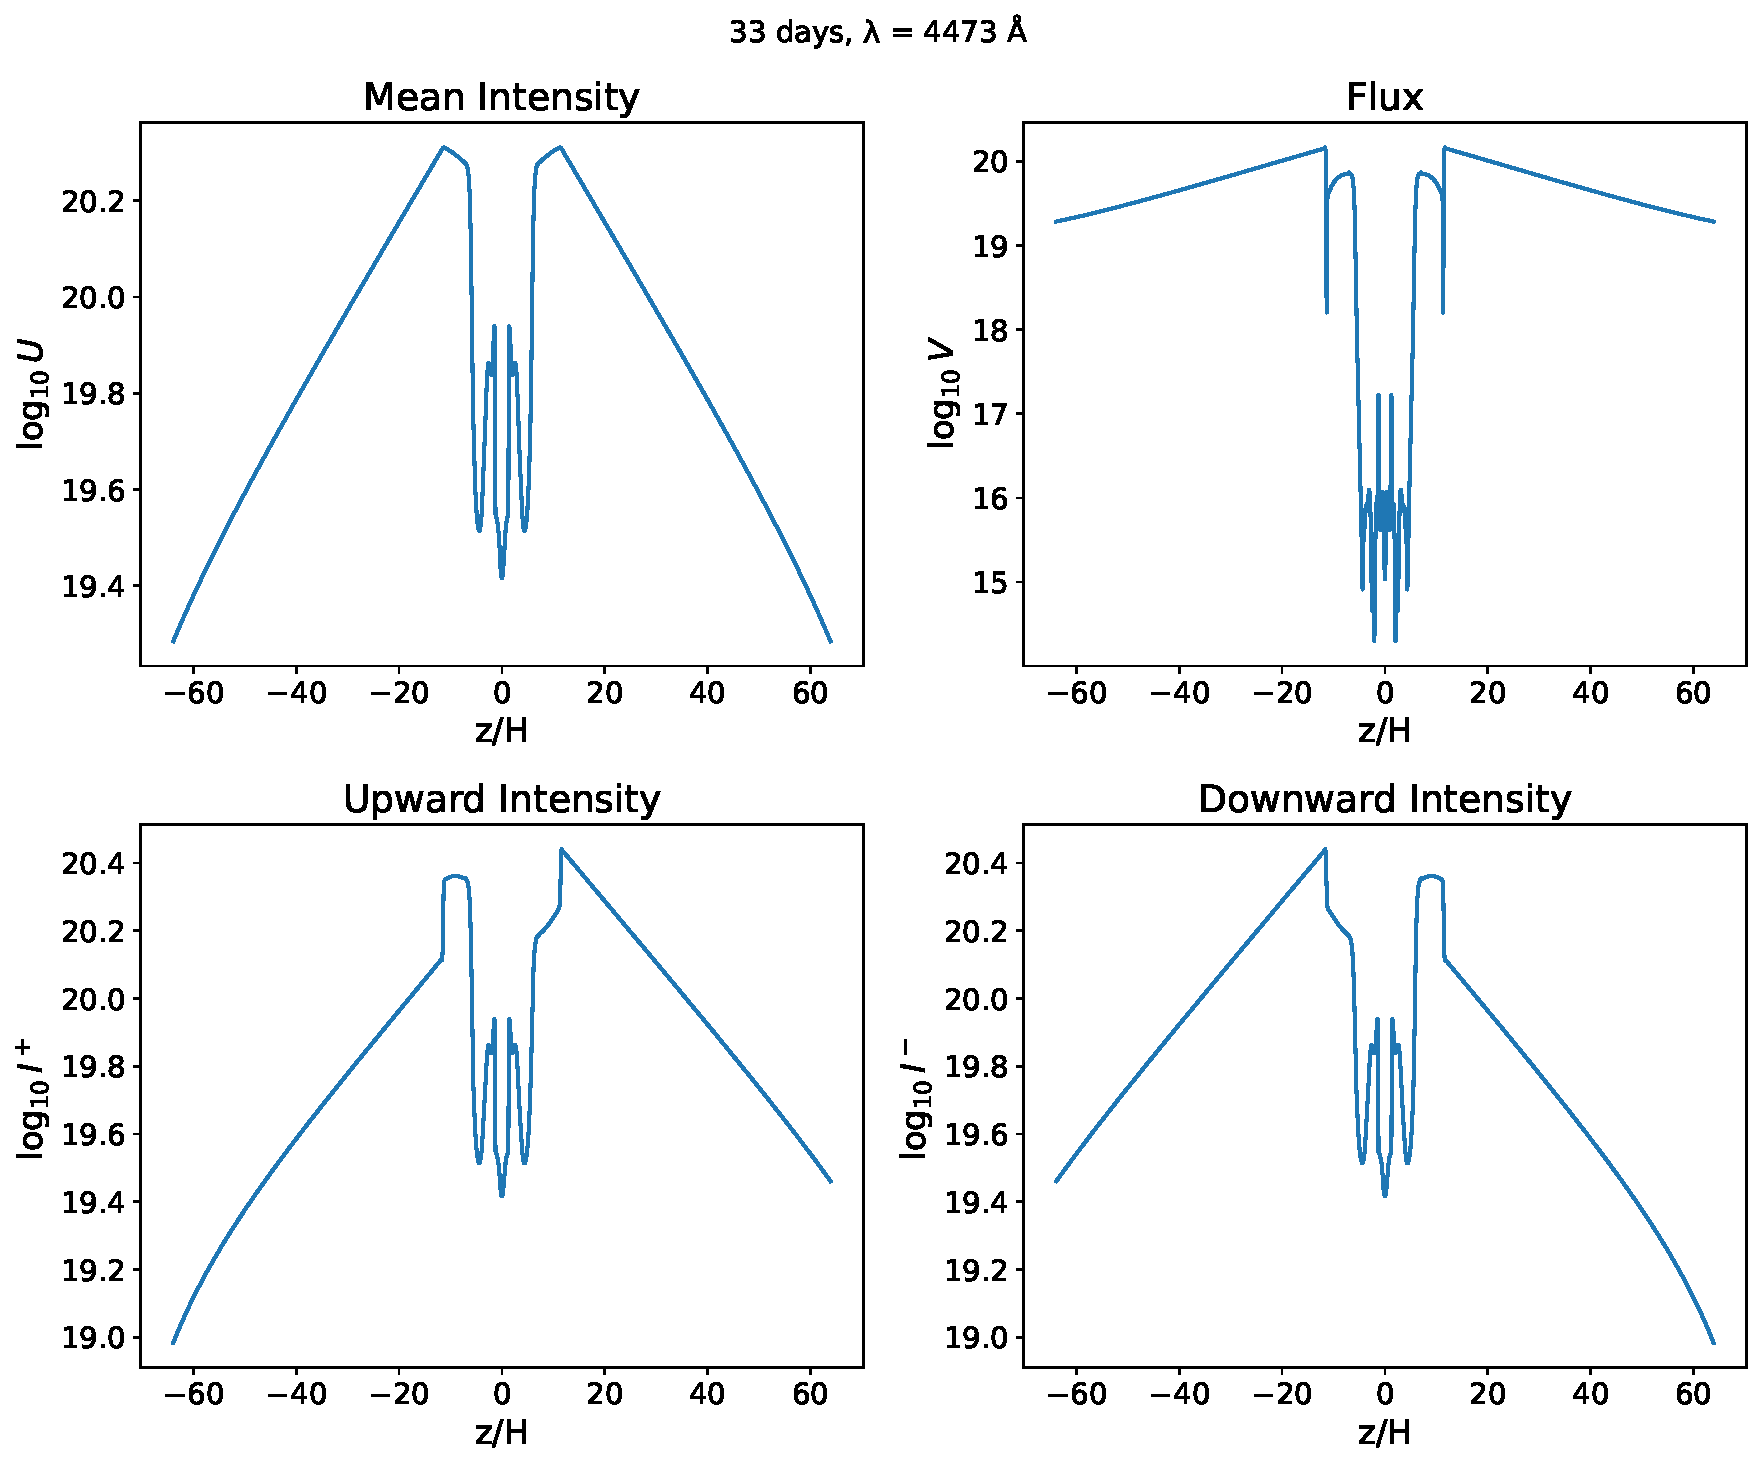
\includegraphics[width=1\textwidth]{ch_snrt_figs/intensity_480x480_w4473_0013.pdf}
	\caption[Feautrier Solutions from \ocotillo for the fiducial model \texttt{r1e3\_z0h} at 33 days]{Mean intensity, flux, and intensity results at shock breakout.}
	\label{fig:UVIpIm-13}
\end{figure}

\begin{figure}
	\centering
	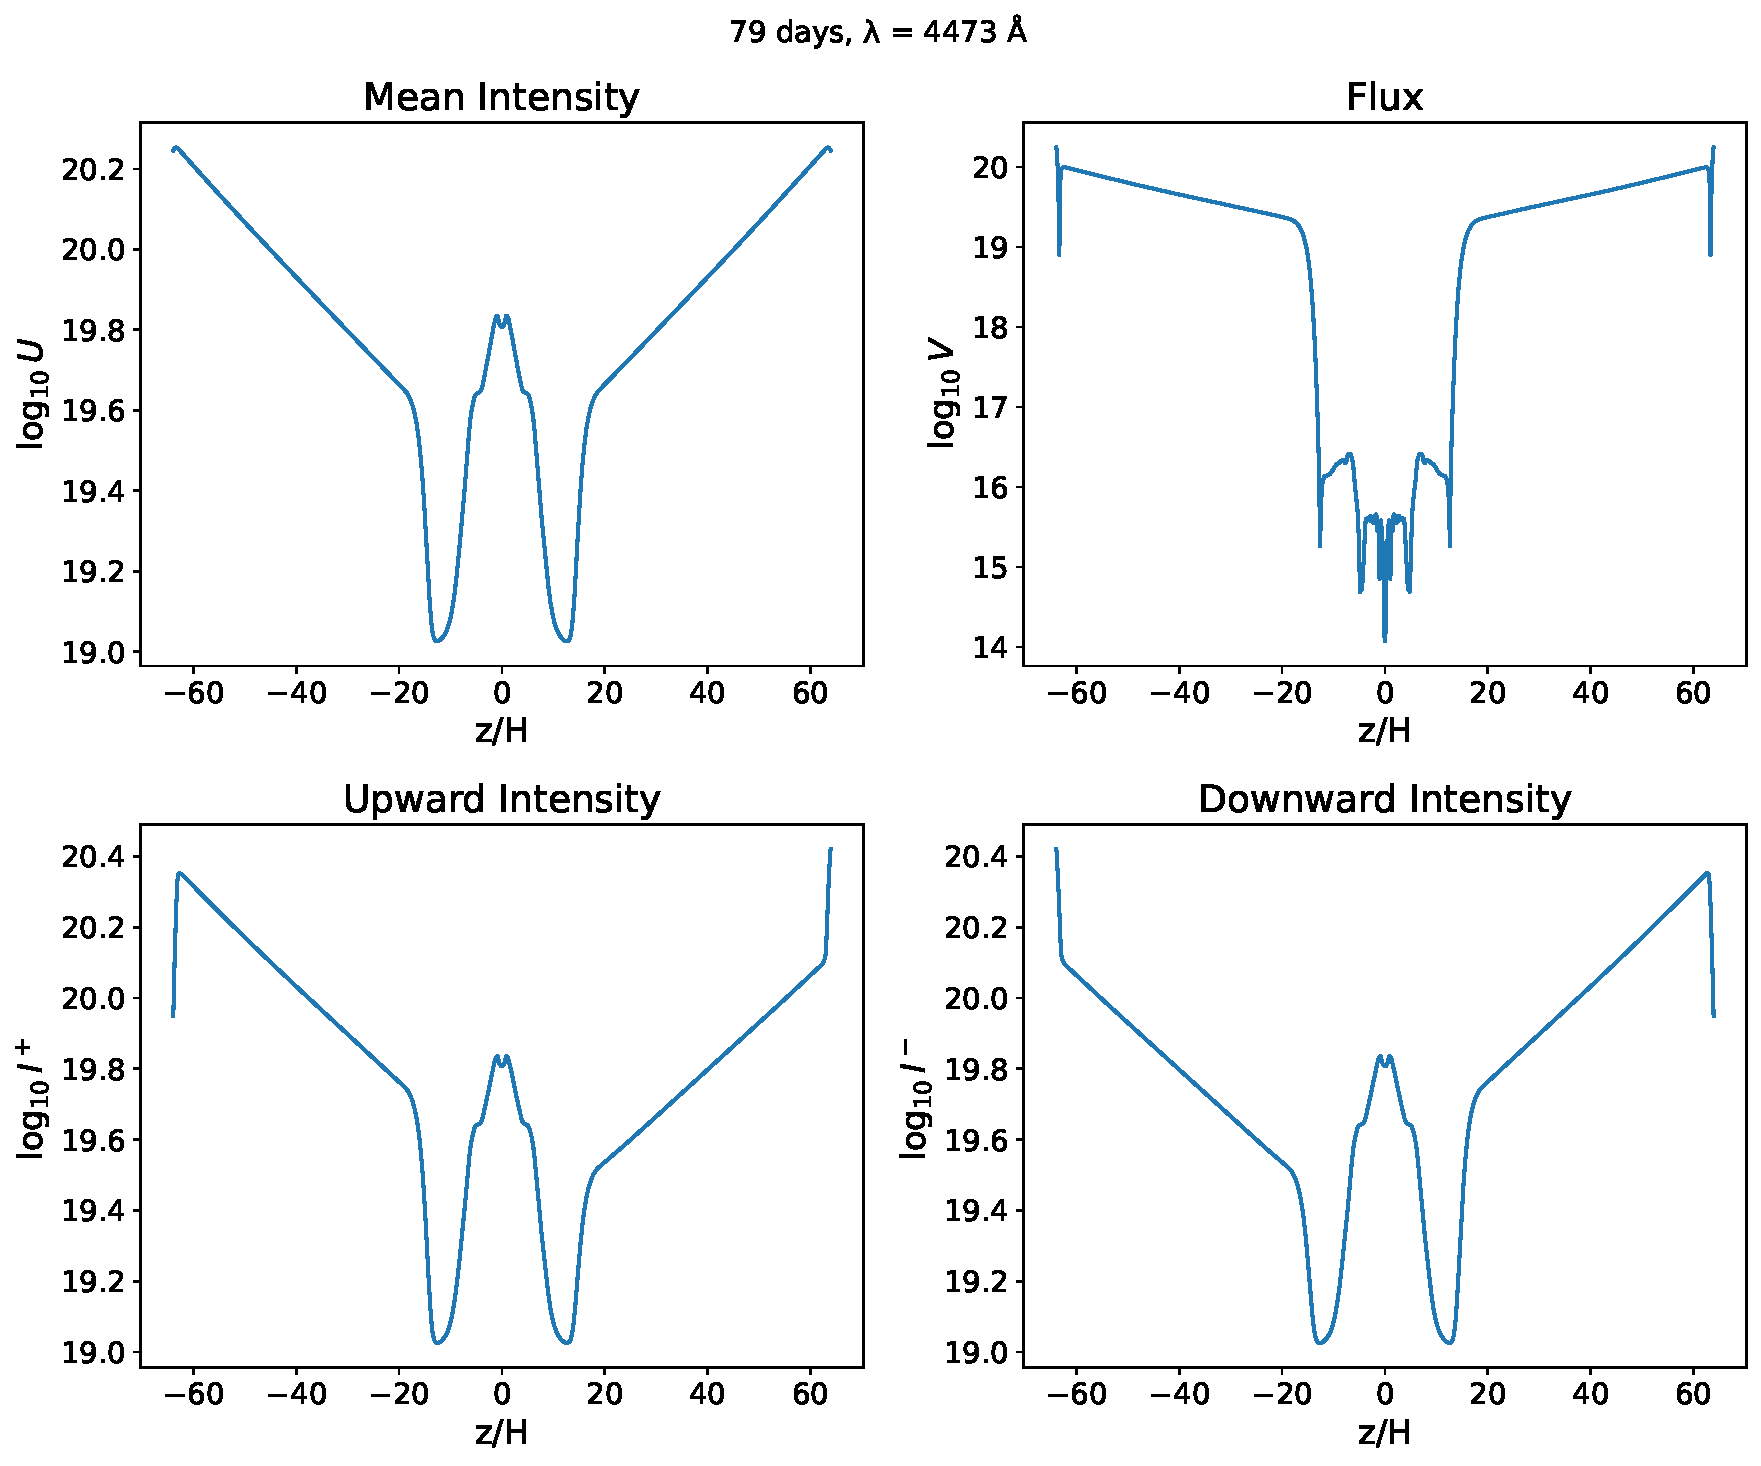
\includegraphics[width=1\textwidth]{ch_snrt_figs/intensity_480x480_w4473_0031.pdf}
	\caption[Feautrier Solutions from \ocotillo for the fiducial model \texttt{r1e3\_z0h} at 79 days]{Mean intensity, flux, and intensity results in the snapshot before the shock leaves the domain.}
	\label{fig:UVIpIm-31}
\end{figure}


\subsection{Results} \label{sec:results}

\subsubsection{Fiducial Model} \label{sec:fiducial-results}

The \citet{SirkoGoodman03} disk has the highest volume density at $10^3\,\Rs$ where we place our fiducial miplane model \code{r1e3-z0h}.
This location was also chosen because it is the most optically thick and thus most likely to prevent or delay electromagnetic radiation from reaching the disk photosphere.
Using \eq{eqn:temp-profile} to apply the temperature profile, we set $\Tmid=6\times10^4$ K.
The blue curve in Fig.~\ref{fig:all_lcs} is the light curve calculated using our post-processing radiative transfer code \ocotillo
%\ref{sec:Appendix-RTModel})/
after integrating the flux over 50 wavelengths over the range $800\leq\lambda\leq8000\ \text{\AA}$.
The light curve remains constant for the first $\sim$20 days when the shock begins to pass through the disk's photosphere and breaks free at $\sim$30 days.
The luminosity rises to $10^{46}\,{\rm erg\,s}^{-1}$ over the next 50 days as the shock expands outside the disk, peaking at $\sim90$ days.
The kink in the light curve at this time is due to the shock crossing the $z$-boundary, meaning we do not capture the true peak of the lightcurve.
However, continuing their curves, we can estimate their peaks will occur at 115 days emitting $2\times10^{47}\,\text{erg s}^{-1}$ (\code{r1e3-z1h-up}) and at 140 days emitting $3\times10^{46}\,\text{erg s}^{-1}$ (\code{r1e3-z0h}).

\begin{figure}[htbp]
    \begin{subfigure}{0.5\textwidth}
        \centering
        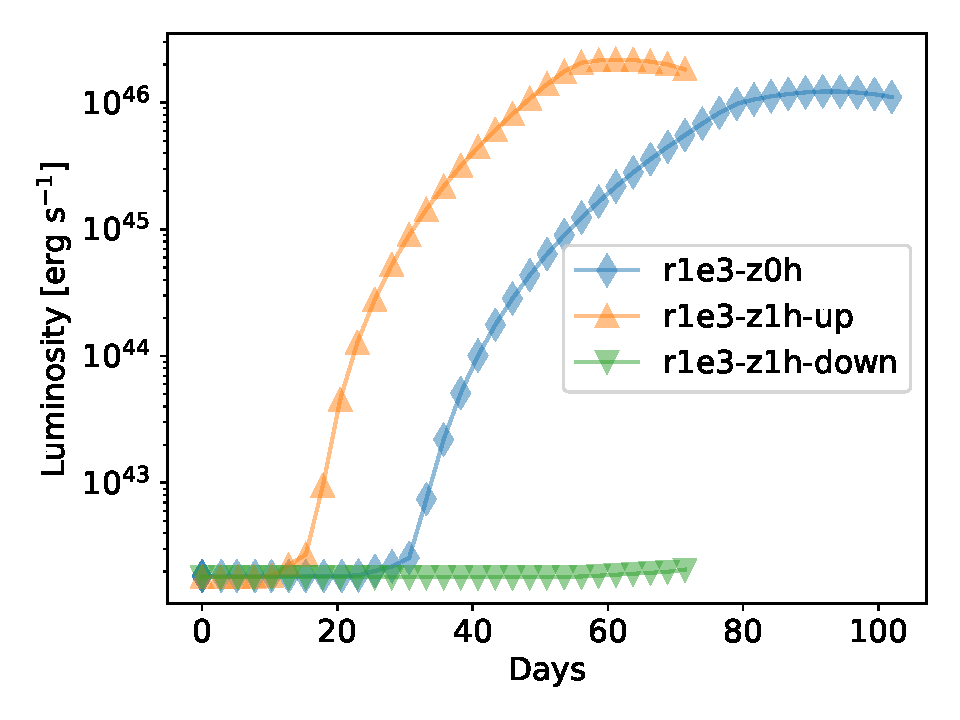
\includegraphics[width=1\linewidth]{ch_snrt_figs/lightcurves_r3.pdf}
    \end{subfigure}
    \begin{subfigure}{0.5\textwidth}
	\centering
        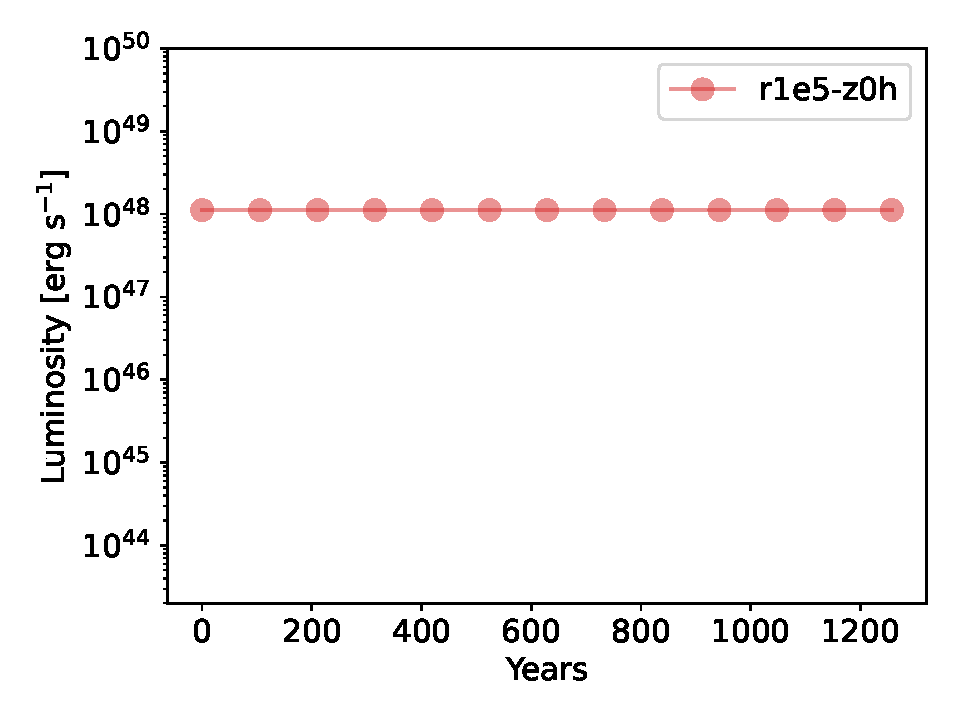
\includegraphics[width=1\linewidth]{ch_snrt_figs/lightcurves_r5.pdf}
    \end{subfigure}
	\caption[Optical light curves]{\textbf{Optical light curves} for our SN simulations integrated over 50 wavelength bins spanning 800 to 8000 $\text{\AA}$.
	\code{r1e3-z0h} is our midplane fiducial model at $r=10^3\,\Rs$, \code{r1e3-z1h} is our model at the same radius but with the SN placed at a height $z=1\,H$.
	The curve labeled with \code{-up} is produced when observing from the positive $z$ boundary (i.e., the same side of the midplane as the offset SN), while the curve labeled with a \code{-down} is produced when observing from the negative $z$ boundary, or the far side of the disk.
	The lower panel shows the lightcurve from our \code{r1e5-z0h} model which places a midplane SN at $r=10^5\,\Rs$.
    % The radiation from the midplane supernova (solid line) escapes the optically thick disk after $\sim$30 days, and the luminosity rises over the next 60 days and peaks at $10^{46}$ erg s$^{-1}$. 
    }
    \label{fig:all_lcs}
\end{figure}

\subsubsection{Offset Model}

Our model where the SN is placed at $z=1\,H$ produces two different light curves when viewed from opposite sides of the disk.
When viewed from the same side of the midplane as the SN (model \code{r1e3-z1h-up}) the orange light curve exhibits changes earlier than the default midplane case, corresponding to the shorter time it takes the shock to reach the disk photosphere.
Now, the radiation escapes at $\sim15$ days and rises faster than the midplane case in \code{r1e3-z0h} to a peak twice as bright.
Viewing from the far side of the disk (model \code{r1e3-z1h-down}), the green light curve shows no change except for a slight brightening when the flow reaches the disk photosphere near $\sim60$ days.

\subsubsection{SNe in the Outer Disk}

The right panel of Fig.~\ref{fig:all_lcs} shows the lightcurve for model \code{r1e5-z0h} where a midplane SN is placed at $r=10^5\,\Rs$.
In Paper I, the shock from this SN did not break free from the disk, and we see that the light curve similarly remains constant.
The baseline luminosity for the disk in this lightcurve is higher than the other light curves due to the hotter effective temperature of the disk at $r=10^5\,\Rs$. 

% Text for the color evolutions.
% The right panel shows the color evolution when comparing the central wavelengths in the $g$ and $r$ filter bands. The color becomes bluer as the bright shock dominates the dimmer disk. However, the color only changes by 0.04 -- well within the scatter of the ZTF data for AGN J1249$+$344.


\subsubsection{Color Evolution}
SNe are often classified and identified by their color evolution.
We integrate the flux emitted by our models over the wavelength ranges corresponding to the ZTF $g$ and $r$ band filters and calculate the $g-r$ color evolutions with:
\begin{align}
	F_{i} &= \int_{\lambda_{i}^0} ^{\lambda_{i}^1} F_\lambda d\lambda \\
	g-r     &= -2.5\log_{10}\frac{F_g}{F_r}
\end{align}

\Fig{fig:color-lightcurve} shows the color evolution for each of the models.
For models \code{r1e3-z0h} and \code{r1e3-z1h-up}, the color becomes slightly bluer when the hot shock emerges and remains constant as the ejected material expands.
Meanwhile, models \code{r1e3-z1h-up} and \code{r1e5-z0h} do not appreciably change color, mimicking their light curves, but \code{r1e3-z0h-down} does slightly change as the subsonic flow breaks through to the far side.
Even though two models showed color changes, the difference is small $\Delta (g-r)=0.04$ and would not have been detectable against the variability in AGN J1249$+$344 ($\Delta(g-r)\sim0.1$) if alert ZTF19abanrhr had been caused by a SN.

\begin{figure}
    \centering
    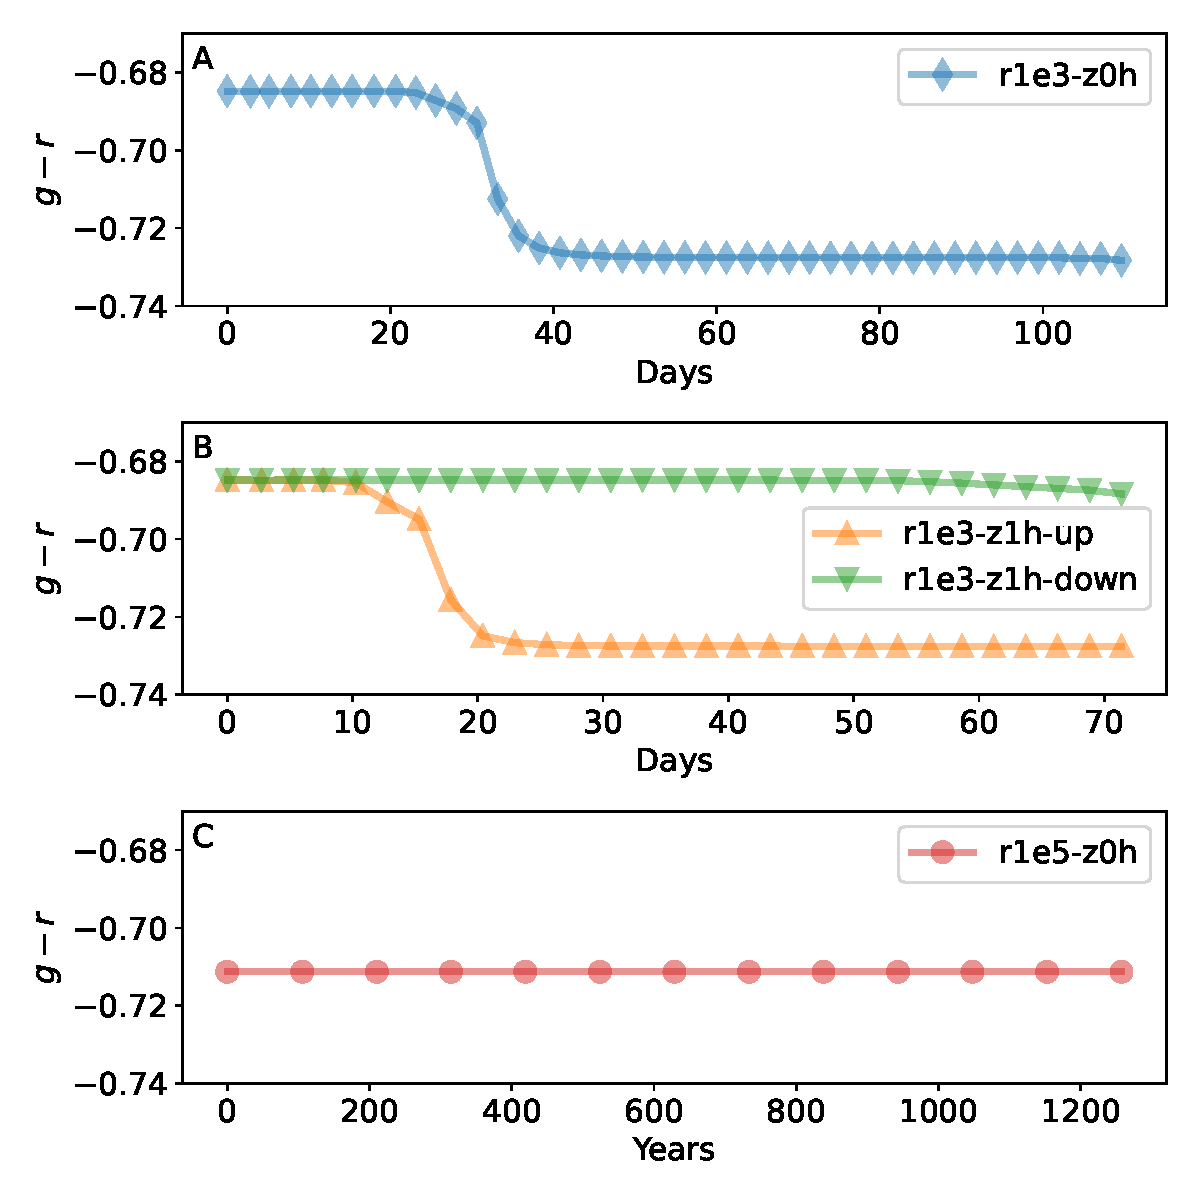
\includegraphics[width=1.0\columnwidth]{ch_snrt_figs/gr_color_composite.pdf}
	\caption[ZTF $g-r$ color evolutions]{ZTF $g-r$ color evolutions. Panel A is from our fiducial model at $R=10^3\,\Rs$, panel B is the offset model at the same radius, and panel C is the midplane model at $R=10^5\,\Rs$.
    The observed color becomes bluer when the shock breaks free, but the small change $\Delta(g-r)\sim 0.04$ would be undetectable amidst the noise for AGN J1249$+$344 with $\Delta(g-r)\sim0.1$ as reported by \citet{Graham+20}.}
    \label{fig:color-lightcurve}
\end{figure}


% \subsection{Magnitudes and Colors} \label{subsec:Mags+Colors}


% According to the methods described in the previous subsection, we derived a multi-wavelength flux $F_\lambda$ from our simulation. In order to compare them with the lightcurves quoted in \citet{Graham+20}, we convert the flux into apparent magnitudes.
% $F_\lambda$ is the value observed by a telescope placed directly at the z-boundary of the computational domain, so we convert these to apparent magnitudes for a source in AGN J124942.3 $+$ 344929 at $z=0.438$ or ~2.4 Gpc \citep{Graham+20}.

% To calculate a bandpass magnitude requires the zero point. ZTF filters are calibrated to match the Pan-STARRS 1 filters according to the release paper \citep{Bellm+19}. Magnitudes in this system follow the "monochromatic AB magnitudes" (Oke \& Gunn 1983)

% \begin{align}
% m_{\rm ABNU}(\nu) &= -2.5\log(f_\nu/3631\ {\rm Jy}) \\ 
%             &= -48.6 -2.5\log(f_\nu[{\rm erg/sec/cm}^2{\rm /Hz}])
% \end{align}
% \citet{Schlafly+12} reported zero points of $g_{\rm ZP}=24.41$ and $r_{\rm ZP}=24.68$, which we can use to calibrate the flux to those of the observations in \citet{Graham+20}.

\subsection{Discussion} \label{sec:discussion}

The baseline disk luminosities in Fig.~\ref{fig:all_lcs} are only produced by the radiation emitted by the small patch of the disk contained in the shearing box models, whereas the full integrated disk luminosity is much larger.
While studying spectra for AGN accretion disks, \citet{Hubeny+01} found that a disk around a black hole of mass $\Mbh=10^8\,\Msun$ has a luminosity $L=0.3L_\text{Edd}=4.4\times10^{45}(M/\Msun)$ erg s$^{-1}$ when considering electron scattering and a viscocity parameter of $\alpha=0.01$ .
Therefore, only the SNe in models \texttt{r1e3-z0h} and \texttt{r1e3-z1h-up} may be detectable against the bright disk, and any observations would need to be able to distinguish changes from the disk emission by a factor of a few.
Additionally, as shown in \Fig{fig:color-lightcurve}, the color changes for these two SNe are very small ($\Delta g-r \sim 0.04$).



Comparing with alert ZTF19abanrhr, the proposed EM counterpart to GW190521, our lightcurves are similarly energetic, and exhibit the same lack of color evolution.
Therefore, an AGN-SN may be indistinguishable from a flare caused by the recoiling remnant of a BBH merger that generates a shock in the disk \citep{McKernan+19}. 
Future work should model the black hole recoil to identify distinguishing characteristics between the two events.

While the light curves do begin to level out, the peaks we see in the \code{r1e3-z0h} and \code{r1e3-z1h-up} curves in \Fig{fig:all_lcs} are artificially caused by the shock passing through the $z$ boundaries.
We cannot push our domain size larger using the current grid structure due to resolution limitations without needing non-equidistant grids,  mesh refinement, or global simulations in polar coordinates.
Also, our radiative transfer model is limited to one dimension, and therefore cannot account for scattering at oblique angles to the line of sight.
As such, the mean intensity may change due to this effect, but we have performed these calculations with a face-on view of the disk which is expected to be the brightest viewing angle.
However, massive stars in the disk may not detonate as SNe at all.
The disk is a large reservoir of hydrogen fuel that continuously replenishes the star's supply if it is sufficiently embedded in the disk.
\citet{CantielloJermynLin21} showed that stars can reach masses of $M\approx300\,\Msun$, easily passing through the so-called pair-instability mass gap that spans $60\lesssim M \lesssim 160\,\Msun$ \citep{WoosleyHeger21}.
Stars that reach these masses will need to expel much more massive envelopes that could significantly delay their shock breakout from the disk or turn it into a subsonic flow entirely.
Thus massive stars that do finally fuse iron in their cores while embedded in an AGN disk will likely not evolve the same as those that lived their lives in the field away from such a plentiful resource.

%\begin{itemize}
%    \item observable against AGN disk luminosity? (draw line next to LCs?)
%    \item how do SNe impact broad line region (BLR) of AGN?
 %   \item Are repeated SNe required to physically perturb the disk enough for the  BLR to change (check paper I for discussions of the broadline region)?
 %   \item can SNe create hot spots that result in BLR variability?
 %   \item rates of these SNe given the star formation rate in the outer disk \citep{SirkoGoodman03, DittmanMiller20} and disk capture \citep{Fabj20}. Need to consider that stars possibly evolve differently in AGN due to its large fuel reservoir \citep{Cantiello21}.
%\end{itemize}


\subsection{Conclusions} \label{sec:conclusion}

We performed post-processing radiative transfer calculations on hydrodynamic shearing box calculations of SNe embedded in AGN disks.
By implementing the Feautrier method we calculated the absorption and scattering processes caused by hydrogen atoms and free electrons.

For SNe at the midplane in the inner disk ($r=10^3\,Rs$), the radiation emerges $\sim30$ days later and rises quickly to a peak at $L=10^{46}\ \text{erg s}^{-1}$.
Typical AGN luminosities can be $\mathcal{O}(10^{43}-10^{48}\ \text{erg s}^{-1})$, so these SNe will only be brighter than AGN of $L\ll10^{46}\,\text{erg s}^{-1}$, which is the range for Seyfert galaxies and other low-luminosity AGN, and will not be visible in quasars.
Radiation from a SN at the same location but offset from the midplane at $z=1\,H$ emerges 15 days earlier, rises much faster, with a luminosity that peaks at $2 \times 10^{46}\,\text{erg s}^{-1}$ when viewed from the same side of the midplane.
The radiation does not reach the other side of the disk in a detectable manner under this scenario.
While bright, these SNe may not be detectable against a bright AGN disk, but would be easily seen if occurring in a starved disk or during an episode of lower mass accretion rates.
For SNe detonating in the outer disk at $r=10^5\,\Rs$, the large scale height of the disk prevents the hot shock from emerging from the photosphere.

Embedded SNe do not exhibit a significant color evolution.
Without this key indicator that is common to naked SNe, they may be indistinguishable from flares produced by recoiling BBH merger remnants.
As such we will need to consider a different part of the spectrum or aspects of these transients to reliably distinguish between flares emitted by embedded merger remnants versus embedded SNe in transient searches such as ZTF or LSST and their archives.

